\documentclass[a4paper,10pt]{article}
%\documentclass[a4paper,10pt]{scrartcl}
\usepackage[spanish]{babel}
\usepackage[utf8]{inputenc}
\usepackage{amssymb, amsmath, amsbsy}
\usepackage{cancel} % para tachar
\usepackage{mathdots} % para el comando \iddots
\usepackage{mathrsfs} % para formato de letra
\usepackage{stackrel} % para el comando \stackbin
\usepackage{graphicx}
\graphicspath{ {images/} }

\title{Identificar las aplicaciones de los manipuladore paralelos}
\author{Gutiérrez Muñoz José de Jesús \\ 7 - A \\ Ing. Mecatrónica}
\date{5 - Noviembre - 2019}
\begin{document}
\maketitle

Manlipulador paralelos.

Es un dispositivo multifuncional y manipular materiales, partes o herramientas a través de movimientos programados variables para las realización de una variedad de tareas especificadas.

Un robot paralelo está compuesto por una cadena cinemática cerrada, la cual consta de cadenas seriales separdas que concectan al eslabón fijo (plataforma fija) o eslabón movil (plataforma móvil).

Los robots también son llamados manipuladores, y ambos términos son manejados en este trabajo.

Aplicaciones iniciales.

Un robot paralelo consiste de una plataforma móvil unida a una plataforma fija mediante una serie
de cadenas cinemáticas llamadas piernas. Partiendo del anterior concepto, Bonev establece que el
origen del robot paralelo se encuentra en la industria del entretenimiento, siendo James E. Gwinnett en
el año 1928 uno de los pioneros en patentar un artefacto basado en el concepto de robot paralelo. La
Figura 1 presenta un esquema incluido en el documento de la patente original.

El dispositivo 
presenta una arquitectura donde una cadena cinemática o pierna central restringe el movimiento de la
plataforma móvil respecto a la base de forma tal que su movimiento resultante es del tipo esférico. Una
cadena cinemática ubicada en uno de los extremos de las plataformas, provee el movimiento de rotación
a la plataforma móvil que es aprovechado para producir el movimiento requerido para el entretenimiento
de los usuarios.

\begin{center}
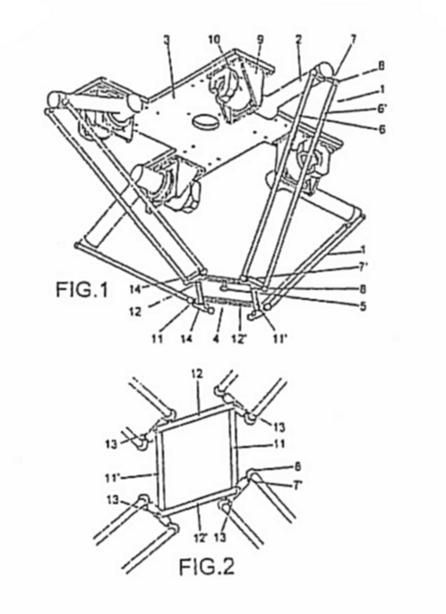
\includegraphics[width=\textwidth]{Imagen1.jpg}
\end{center}

La primera aplicación industrial conocida del robot paralelo, siguiendo la cronología propuesta por
Bonev, fue presentada por Willard L.V. Pollard en el año 1940 [4]. El dispositivo fue propuesto para
pintar vehículos de forma automática con pintura de aerosol y posteriormente fue patentado como
dispositivo para controlar el posicionamiento de una herramienta [5]. La Figura 2 muestra una
representación esquemática del ingenioso aparato de 5 grados de libertad (GdL) donde la plataforma
móvil va unida a la fija mediante 3 cadenas cinemáticas o piernas. El diseño presenta tres motores que
determinan la posición de la cabeza de la herramienta, y otros dos motores que mediante un sistema de
cables transmite el movimiento que permite orientar la herramienta.

Más tarde en la década de los 50, Eric Gough un ingeniero automotriz trabajando en la fábrica de
neumáticos de la Ford Dunlop en Birmingham, Inglaterra, desarrolla una máquina Universal de pruebas
de neumáticos. La plataforma fue puesta en funcionamiento en el año 1954 y cumplía la función de
probar mecánicamente neumáticos mediante la aplicación de cargas combinadas. La Figura 3 muestra
una imagen del dispositivo utilizado por la empresa Dunlop hasta el cierre de la fábrica en el año 1980.
Actualmente el dispositivo se ubica en el Museo de Ciencia de Londres, específicamente en el almacén
Wroughton. Su diseño presenta una forma de octaedro donde cada cadena cinemática es impulsada por
actuadores lineales. El mecanismo presenta 6 GdL.

No fue sino hasta 1965 que aparece la primera publicación científica referida a un robot paralelo.
Stewart introduce un robot paralelo de 6 GdL similar al de Gough. Debido al parecido que presenta
la plataforma Stewart con el robot propuesto por Gough hoy en día la configuración del tipo hexápodo
con actuadores lineales se conoce como plataforma Gough-Stewart. Es de destacar que la plataforma
Stewart fue propuesta para aplicaciones de simulador de vuelo. La Figura 4 muestra el robot basado en
el concepto de Stewart desarrollado para un simulador de vuelo de Lufthansa. Es justo también indicar
que Klaus Cappel en 1964 de forma separada, y sin tener conocimiento previo de los trabajos de Gough
y de Stewart, patenta una configuración similar al robot hexápodo como dispositivo para simulación de
movimiento .

Aplicaciones de los manipuladores paralelos.

Aplicaciones:

Este tipo de manipulador presenta grandes ventajas comparado con los manipuladores seriales, como son: mejor estabilidad y precisión, peso ligero, capacidad de manipular cargas relativamente grandes, altas velocidades y aceleraciones, y baja fuerza de actuación.

En la actualidad los robots son parte fundamental de nuestra industria, facilitando la ejecución de múltiples tareas, aumentando la precisión del producto final y disminuyendo tiempos de ejecución.

Además, son muchos otros los ámbitos en los que los sistemas robóticos modernos colaboran, como pueden ser el sector aeroespacial, diversas aplicaciones médicas, industria de los videojuegos, etc. En particular, los denominados manipuladores paralelos han ido adquiriendo en los últimos años una notable relevancia, existiendo numerosas líneas de investigación y proyectos asociados al estudio y desarrollo de este tipo de robots. Sin embargo, en ocasiones, no siempre existe una comunicación bilateral entre industria e investigación, o incluso entre las propias ramas de investigación existentes, de forma que se crea un cierto desconocimiento acerca de los trabajos realizados, los que están en proceso de ejecución y las posibles líneas de trabajo futuras. Por ello, cuando un determinado ámbito del conocimiento alcanza un cierto grado de madurez, conviene reflejar su actual estado de la técnica. En este sentido, los autores del presente artículo realizan una revisión de los campos en los cuales los manipuladores paralelos tienen una especial participación, así como de las líneas de trabajo más activas en el análisis y diseño de estos robots. Asimismo, se citan varias aportaciones con las que los autores del presente trabajo han contribuido.

Hay diferentes tipos de Manimuladores de paraleos, pero al final todos se rigen por algunas reglas para que se puedan identificar o diferencias de otros tipos de manipuladores.

Entre ellos estan los siguientes:

\begin{center}
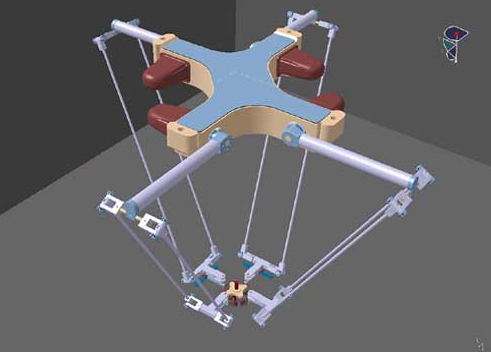
\includegraphics[width=\textwidth]{Imagen2.PNG}
\end{center}

\begin{center}
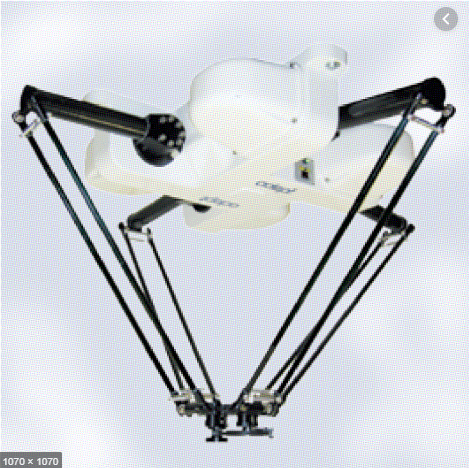
\includegraphics[width=\textwidth]{Imagen3.PNG}
\end{center}

Los robots paralelos se han venido empleando para distintas tareas como en simuladores de vuelo, máquinas caminadoras, dispositivos de máquinas–herramientas, micro manipulación a alta frecuencia (telescopios)y recientemente para tareas de ensamble.

En el sector industrial, donde las velocidades de trabajo y los requisitos son cada vez mayores, se está optando por arquitecturas de mecanismos hasta ahora descartadas. Los manipuladores paralelos han irrumpido en la industria no sin cierto éxito. Su superior capacidad de carga y alta rigidez les permiten ofrecer prestaciones superiores a las de los robots serie en tareas en las que las altas aceleraciones y velocidades son características fundamentales.

Descripción geométrica.

En este trabajo se toma como modelo de estudio una versión del robot Delta integrada por una base fija y otra móvil conectadas por tres cadenas cinemáticas idénticas.

\begin{center}
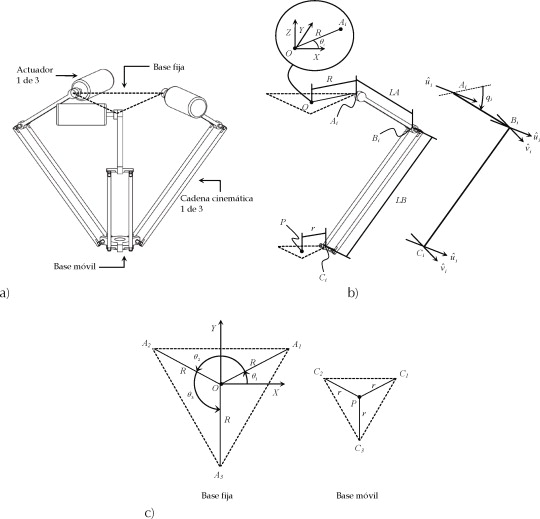
\includegraphics[width=\textwidth]{Imagen4.jpg}
\end{center}

Robot tipo Delta, a) vista general, b) estructura de la i-ésima cadena cinemática, c) configuración geométrica de la base fija y la base móvil.

Como se observa en la figura 1b, un sistema de referencia global (X, Y, Z) se define en el punto O en el centro de la base fija. Los ejes X y Y yacen en el plano de la base fija y el eje Z apunta hacia arriba verticalmente.

\end{document}
